	
\section{Discussion}
As shown in 
		Figure \ref{fig:DApp} \gls{DApp}, a user's transactions on the application is publicly broadcasting to the blockchain. 
		Implementing architecture for blockchain applications \footnote{Although, server blockchain architecture with an abstraction layer resemble traditional applications, other approaches are available such as offline signing with a public node, and client-blockchain in serverless apps and leveraging cloud infrastructure.} adds an third layer to the standard client-server architecture 	\footnote{ \textbf{Signing Transactions}: One approach involves interacting with the JSON RPC interface of the \gls{Ethereum} node from the application to perform all blockchain operations.}.
		 Disadvantages of blockchain data storage include difficult retrieving relevant information (without an abstraction layer, the entire blockchain or a single transaction is returned), users will experience latency before transactions are validated, 	\footnote{For bitcoin, it takes 10 minutes before blocks of transactions are validated (mining process)} and writing to the blockchain is relatively expensive compared to traditional systems. Usage of interfaces such as the JSON RPC and/or cloud hosting 
	 solutions serve as a abstraction layer allowing databases to load publicly available data on the blockchain
	 	 % rewrite later 
	 	 for more efficient user interactions with that information. 

\begin{warpprint}
\begin{figure}[ht]
\begin{adjustbox}{center,max width=1.1\textwidth}
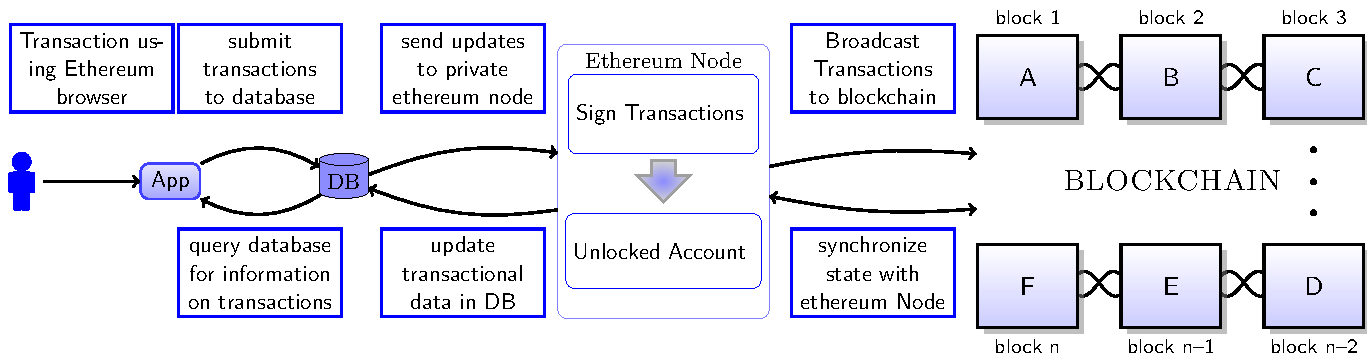
\includegraphics[width=1.2\linewidth]{Diagrams/blockchainInSimpleApp.pdf}
\end{adjustbox}
\caption{An example of server-blockchain architecture in a DAPP.}
\label{fig:DApp}
\end{figure}
\end{warpprint}

\begin{warpHTML}
\begin{figure}[ht]
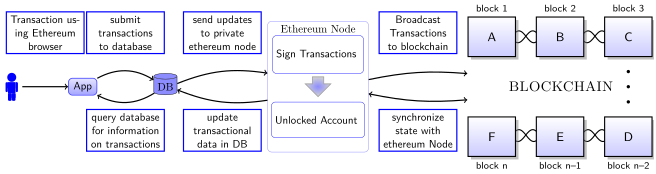
\includegraphics[width=1.2\linewidth]{Diagrams/blockchainInSimpleApp.svg}
\caption{An example of server-blockchain architecture in a DAPP.}
\label{fig:DApp}
\end{figure}
\end{warpHTML}

\begin{warpprint}
\begin{table}[]
\centering
\caption{Sample Decision Matrix for designing a blockchain system}
\arrayrulecolor{white}
\arrayrulewidth=1pt
\renewcommand{\arraystretch}{1.5}
\rowcolors[\hline]{3}{.!50!white}{}
\begin{tabular}{D E A B C }
\multicolumn{1}{l}{}      & \multicolumn{1}{c}{Existing Systems}    & \multicolumn{3}{c}{BlockChain Systems}                                                                                    \\
\multicolumn{1}{c}{Criteria}                 & \multicolumn{1}{c}{Centralized} & \multicolumn{1}{c}{Public} & \multicolumn{1}{c}{Permissioned} & \multicolumn{1}{c}{Private} \\
speed and latency         &                                         &                                       &                                             &                                        \\
scale and volume          &                                         &                                       &                                             &                                        \\
security and immutablity  &                                         &                                       &                                             &                                        \\
storage capacity          &                                         &                                       &                                             &                                        \\
transparency              &                                         &                                       &                                             &                                        \\
\multicolumn{1}{c}{Total} &                                         &                                       &                                             &                                       
\end{tabular}
\end{table}
\end{warpprint}

% HTML VERSION OF TABLE
\begin{warpHTML}

A generic message here? 

\begin{table}
\centering
\caption{My caption}
\begin{tabular}{cllll}
\multicolumn{1}{l}{}      & \multicolumn{1}{c}{Current Solution}    & \multicolumn{3}{c}{Alternative Solutions}                                                                                    \\
Criteria                  & \multicolumn{1}{c}{Centralized Systems} & \multicolumn{1}{c}{Public Blockchain} & \multicolumn{1}{c}{Permissioned Blockchain} & \multicolumn{1}{c}{Private Blockchain} \\
speed and latency         &                                         &                                       &                                             &                                        \\
scale and volume          &                                         &                                       &                                             &                                        \\
security and immutablity  &                                         &                                       &                                             &                                        \\
storage capacity          &                                         &                                       &                                             &                                        \\
transparency              &                                         &                                       &                                             &                                        \\
\multicolumn{1}{l}{Total} &                                         &                                       &                                             &                                       
\end{tabular}
\end{table}
\end{warpHTML}